Für den korrigierten Yield wird zuletzt noch die systematische Unsicherheit bestimmt.
Dabei wird sich in dieser Arbeit rein auf die systematische Unsicherheit, die durch Variation in der Peakextraktion kommt, fokussiert.
Die Variationen die in dieser Arbeit verwendet wurden lassen sich in vier Abschnitte unterteilen.
\begin{figure}[t!]
\centering
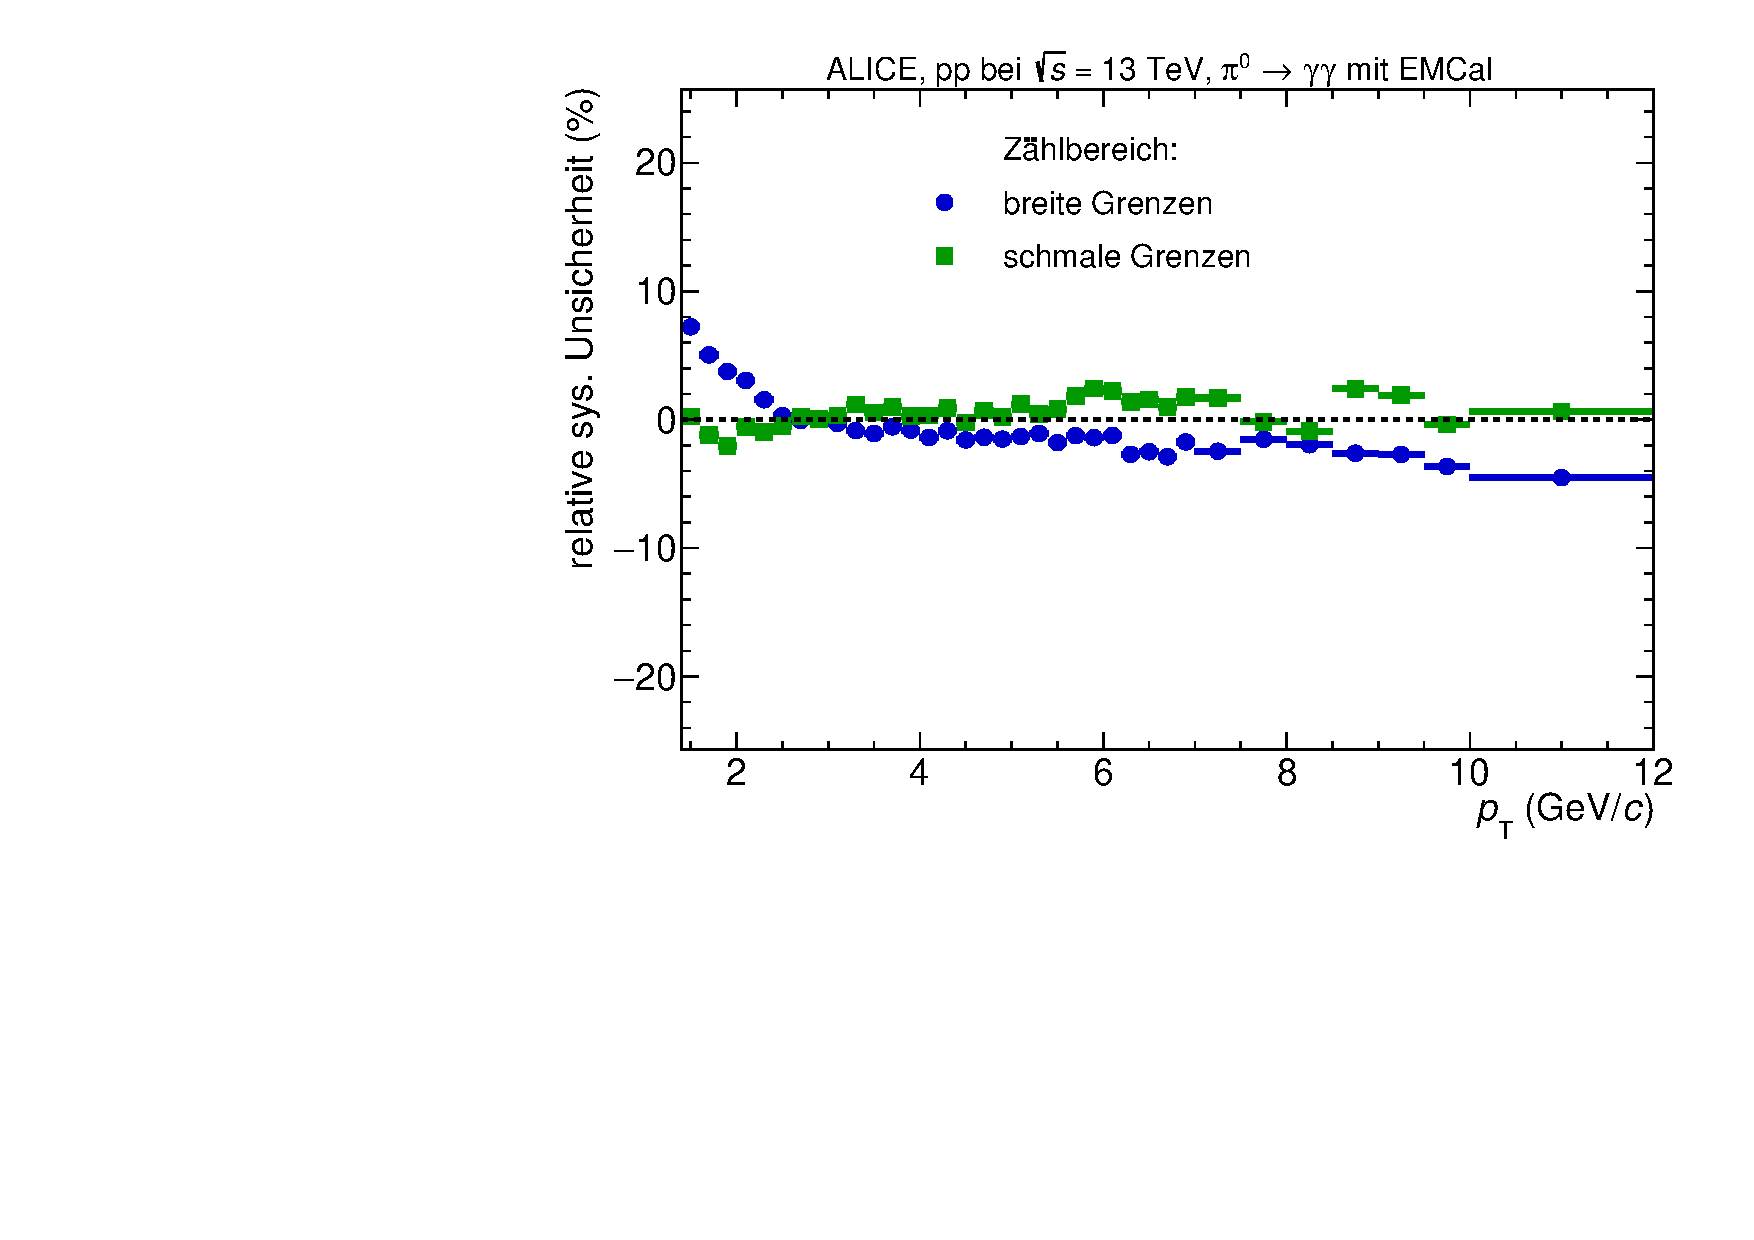
\includegraphics[width=.65\linewidth]{YieldsSysUncerIntRange_Data_2016.pdf}
\caption{Relative systematische Unsicherheit durch die Variation des Zählbereiches abhängig von $p_\text{T}$.}
\label{fig:IntSys}
\end{figure}
\newline
Bei der \textbf{Variation des Zählbereiches}, wird der Zählbereich einmal ausgeweitet und ein anderes mal verkleinert.
Für das Verkleinern wird dabei der untere Wert für $m_\text{inv}$ um $0\,01 \text{ GeV}/c^{2}$ erhöht, während der obere Wert für $m_\text{inv}$ um $0\,025 \text{ GeV}/c^{2}$ verringert wird.
Entsprechend wird beim Ausweiten der untere Wert für $m_\text{inv}$ um $0\,025 \text{ GeV}/c^{2}$ verringert der obere Wert für $m_\text{inv}$ um $0\,025 \text{ GeV}/c^{2}$ erhöht.
\newline
Abbildung \ref{fig:IntSys} zeigt die relative systematische Unsicherheit für die Variation des Zählbereiches. 
%von Andrea, braucht Überarbeitung
Die Abweichungen zeigen sowohl für breite als auch für schmale Grenzen einen annähernd linearen Verlauf, wobei sie im Fall der schmalen Grenzen positiv sind und im Fall der breiten Grenzen negativ. 
%Dabei fallen besonders die ersten Werte für einen vergrößerten Zählbereich auf, da sie vergleichsweise groß sind.
%Diese Werte lassen sich dadurch erklären, dass das kombinierte Template des korrelierten Untergrunds aus dem $p_\text{T}$-Intervall von $1,8 \leq p_\text{T}/(\text{ GeV}/c < 3,2)$.
%Die Anforderung an den Öffnungswinkel bewirkt, dass bei den Templates des korrelierten Untergrunds keine Einträge im Bereich kleiner invarianter Massen vorliegt.
%Durch die Anforderung an den Öffnungswinkel wandert die untere Grenze in der invarianten Masse, ab der es Einträge gibt, mit steigendem $p_\text{T}$ zu höheren $m_\text{inv}$.
Das bedeutet, dass das kombinierte Template des korrelierten Untergrunds für kleine $m_\text{inv}$ nicht den Verlauf der Templates des korrelierten Untergrunds für $p_\text{T} < 1,8 \text{GeV/c}$ wiedergeben kann.
%Die vereinfachte Simulation für die Anforderung an den Öffnungswinkel kann nur verwendet werden um die Anzahl an Einträgen in dem kombinierten Template zu skalieren.
\begin{figure}[t!]
\centering
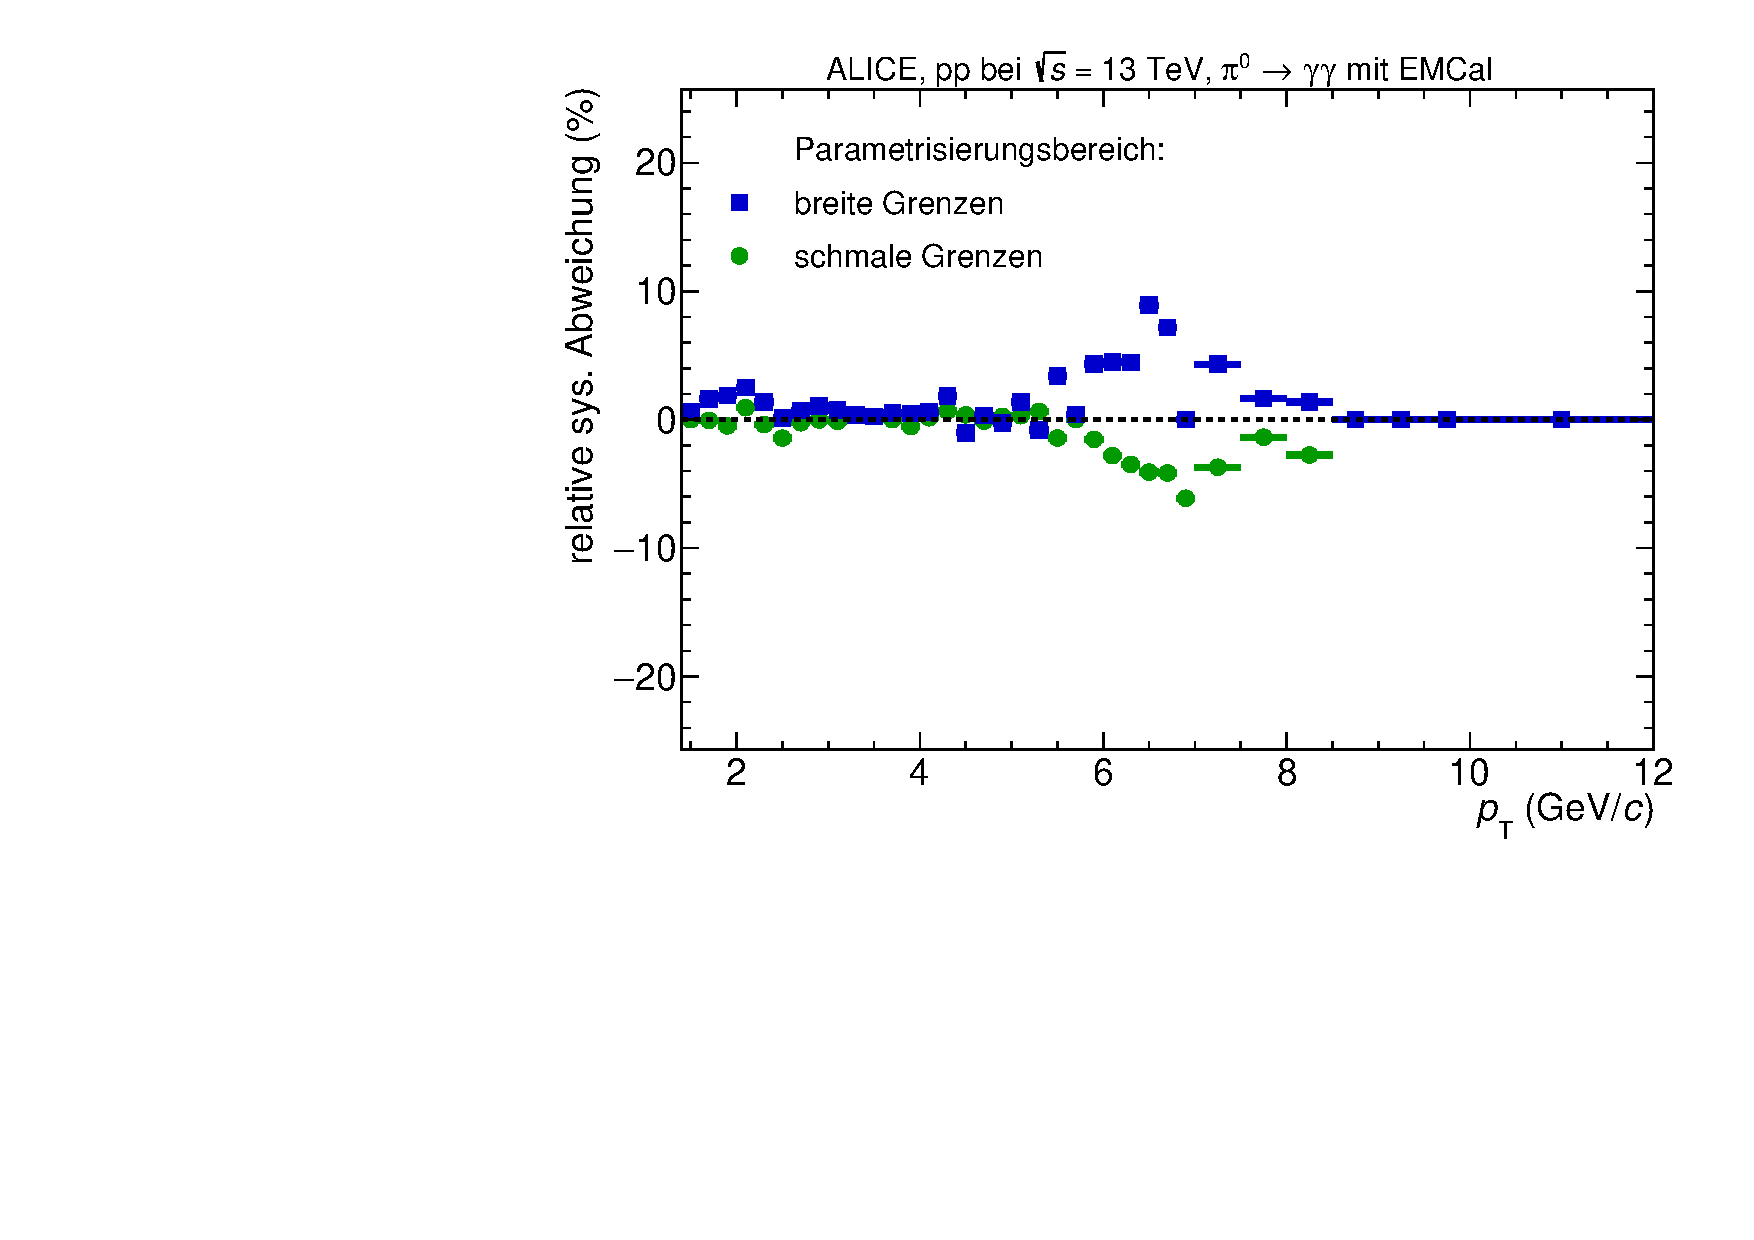
\includegraphics[width=.65\linewidth]{YieldsSysUncerFitRange_Data_2016.pdf}
\caption{Relative systematische Unsicherheit durch die Variation des Paramtrisierungsbereiches abhängig von $p_\text{T}$.}
\label{fig:ParamSys}
\end{figure}
\newline
Bei der \textbf{Variation des Parametrisierungsbereiches} wird analog verfahren, mit den gleichen Zahlenwerten.
\begin{figure}[t!]
\centering
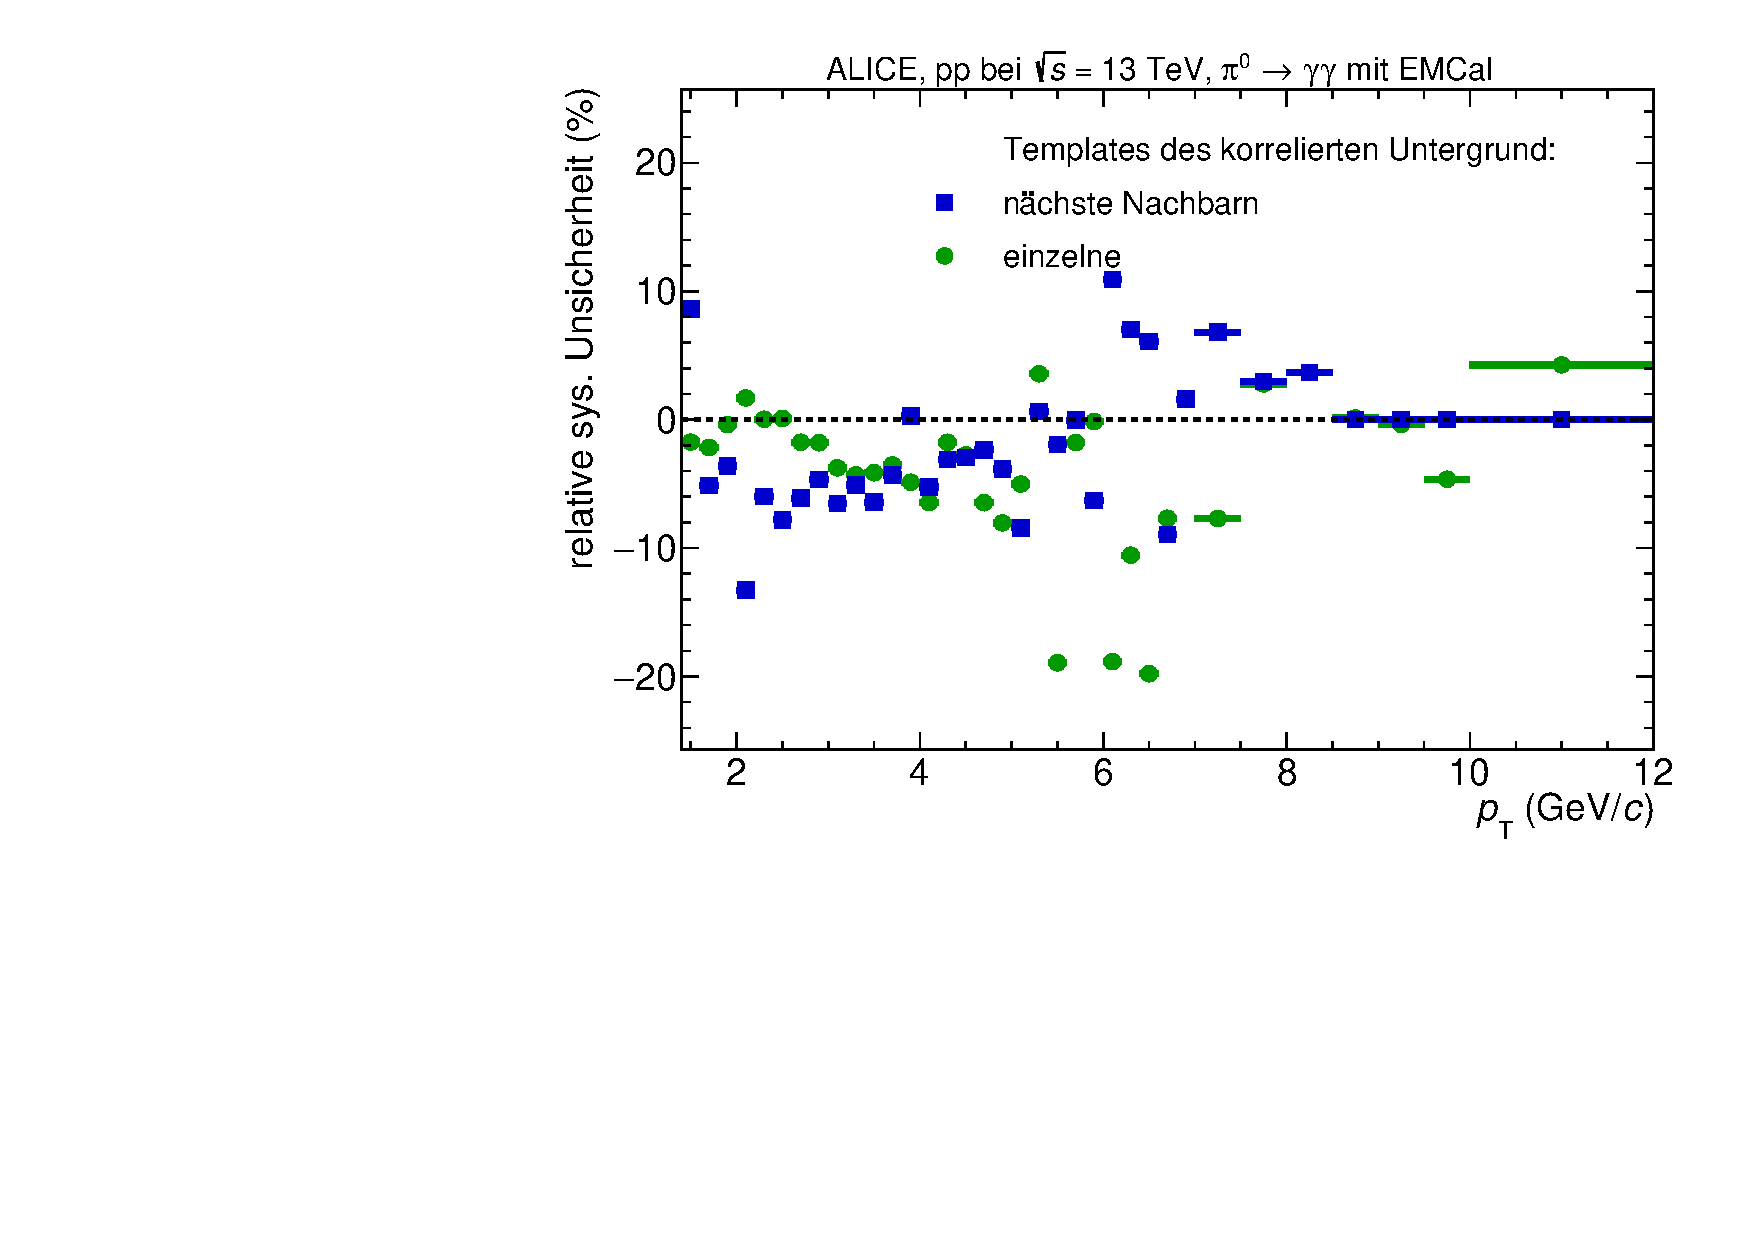
\includegraphics[width=.65\linewidth]{YieldsSysUncerBkgVariation_Data_2016.pdf}
\caption{Relative systematische Unsicherheit durch die Variation der Templates des korrelierten Untergrunds abhängig von $p_\text{T}$.}
\label{fig:BkgSys}
\end{figure}
\newline
Die \textbf{Variation der Templates des korrelierten Untergrunds} basiert auf den in Abschnitt \ref{s3s5s2} vorgestellten Methoden zur Bestimmung der Templates des korrelierten Untergrunds.
\begin{figure}[t!]
\centering
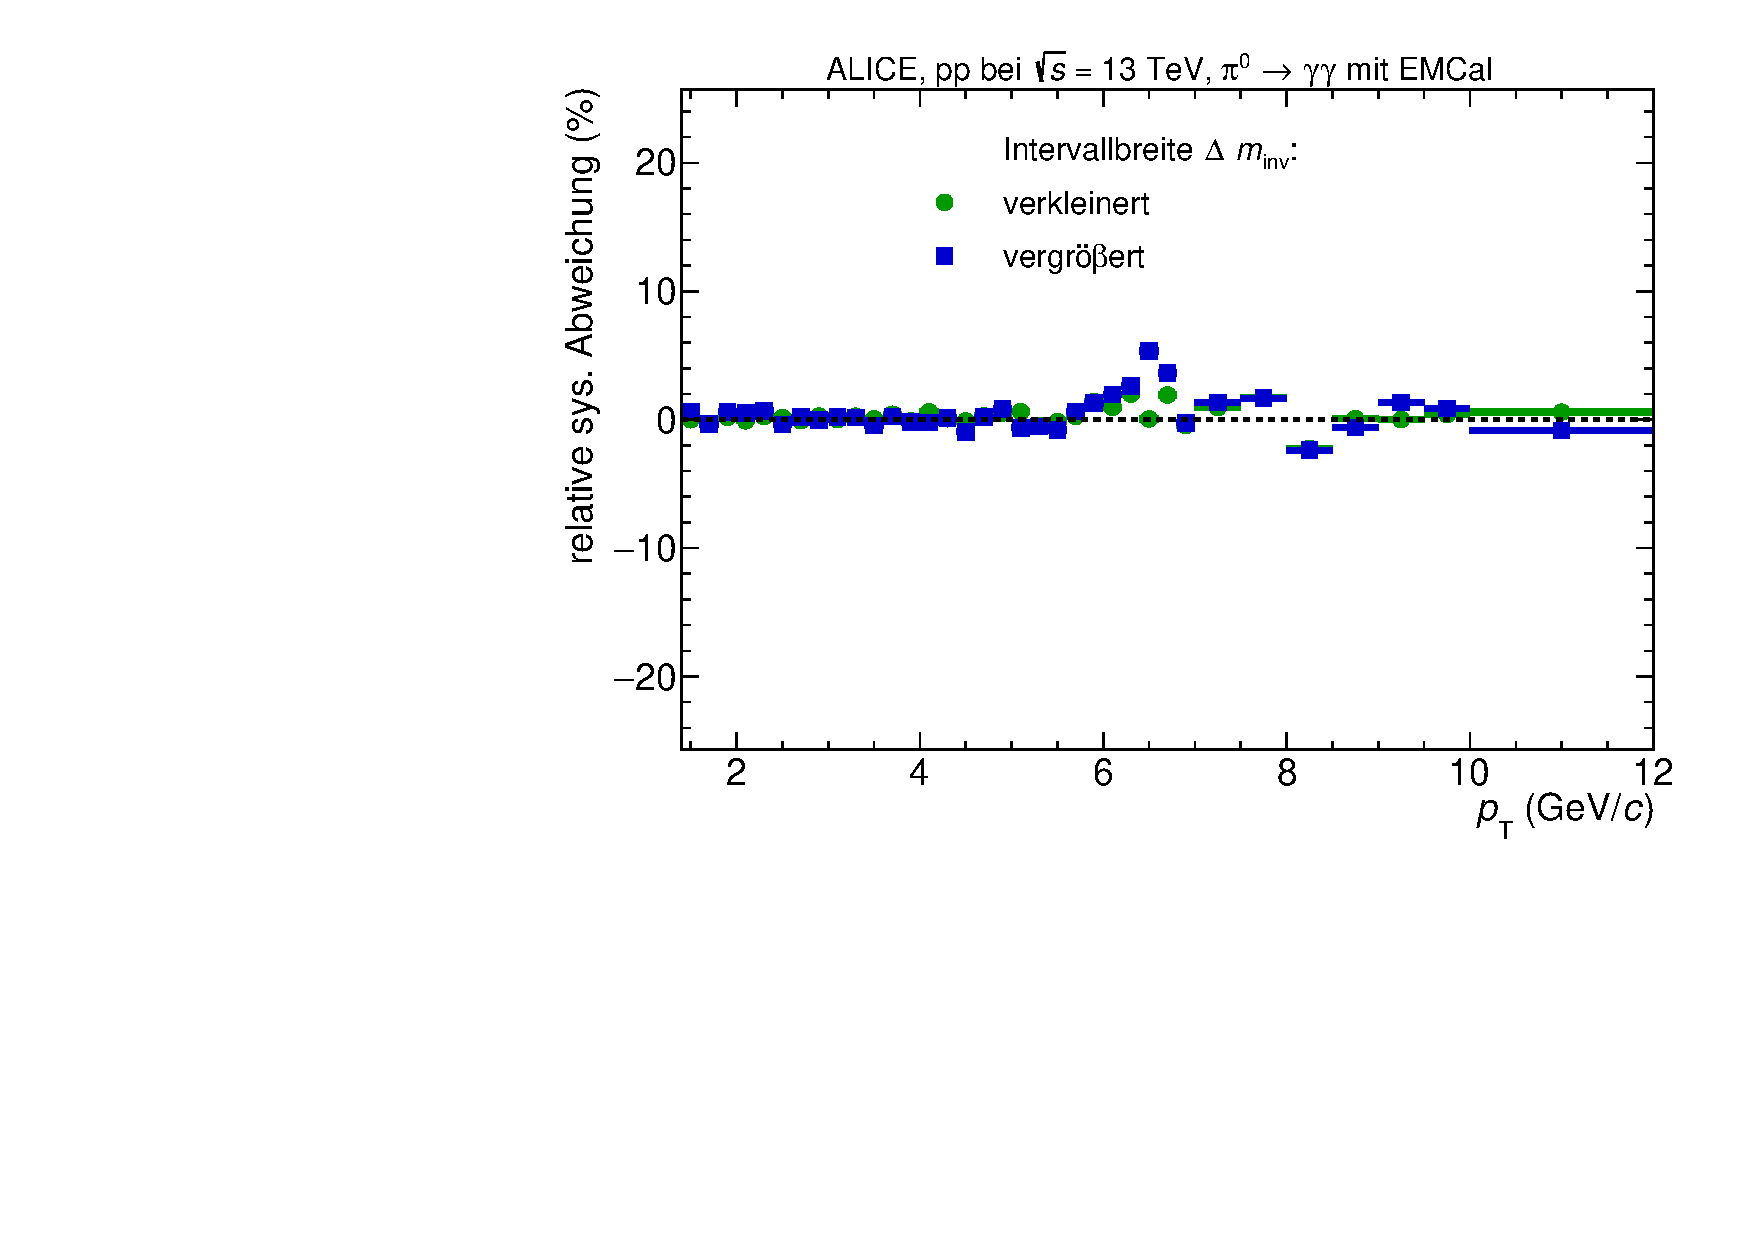
\includegraphics[width=.65\linewidth]{YieldsSysUncerRebinning_Data_2016.pdf}
\caption{Relative systematische Unsicherheit durch die Variation des Rebinnings des korrelierten Untergrunds abhängig von $p_\text{T}$.}
\label{fig:BinningSys}
\end{figure}
\begin{table}[b!]
\centering
\begin{tabular}{c|c|c|}
\cline{2-3}
                                                          & $\Delta m_\text{inv}$ $\left(\text{GeV}/c^{2}\right)$ & $p_\text{T}$-Intervall $\left(\text{GeV}/c\right)$ \\ \hline
\multicolumn{1}{|c|}{\multirow{3}{*}{Standard}}           & $0\,004$                                              & $1\,4-7\,5$                                        \\ \cline{2-3} 
\multicolumn{1}{|c|}{}                                    & $0\,008$                                              & $7\,5-10$                                          \\ \cline{2-3} 
\multicolumn{1}{|c|}{}                                    & $0\,010$                                              & $10-12$                                            \\ \hline \hline
\multicolumn{1}{|c|}{\multirow{3}{*}{Vergr{\"o}{\ss}ert}} & $0\,005$                                              & $1\,4-7\,5$                                        \\ \cline{2-3} 
\multicolumn{1}{|c|}{}                                    & $0\,010$                                              & $7\,5-10$                                          \\ \cline{2-3} 
\multicolumn{1}{|c|}{}                                    & $0\,016$                                              & $10-12$                                            \\ \hline \hline
\multicolumn{1}{|c|}{\multirow{3}{*}{Verkleinert}}        & $0\,002$                                              & $1\,4-7\,5$                                        \\ \cline{2-3} 
\multicolumn{1}{|c|}{}                                    & $0\,005$                                               & $7\,5-10$                                          \\ \cline{2-3} 
\multicolumn{1}{|c|}{}                                    & $0\,008$                                              & $10-12$                                            \\ \hline
\end{tabular}
\caption{Die verschiedenen Breiten der $m_\text{inv}$-Intervalle $\Delta m_\text{inv}$ in Abhängigkeit von $p_\text{T}$.}
\label{tab:Binning}
\end{table}
\newline
Als letztes wird noch die Breite der $m_\text{inv}$-Intervalle $\Delta m_\text{inv}$ in der \textbf{Variation des Rebinnings} verändert.
Die Werte für $\Delta m_\text{inv}$ hängen zunächst von zwei Faktoren ab.
Zum einen werden die Daten für die Analyse in $800$ gleichgroße $m_\text{inv}$-Intervalle aufgeteilt, die von $m_\text{inv} = 0\,0 \text{ GeV}/c^{2}$ bis $m_\text{inv} = 0\,8 \text{ GeV}/c^{2}$ reichen.
Somit beträgt $\Delta m_\text{inv}$ anfangs immer $0\,001 \text{ GeV}/c^{2}$.
Dieser Wert wird vergrößert um die statistische Unsicherheit möglichst klein zu halten, wobei darauf geachtet werden muss, dass es sich bei dem Faktor, um den $\Delta m_\text{inv}$ vergrößert wird, um einen gemeinsamen Teiler von $800$ handelt.
Tabelle \ref{tab:Binning} zeigt $\Delta m_\text{inv}$ im Normalfall, sowie für beide Variationen.
Dabei hängt $\Delta m_\text{inv}$ zusätzlich von $p_\text{T}$ ab.
\begin{figure}[t!]
\centering
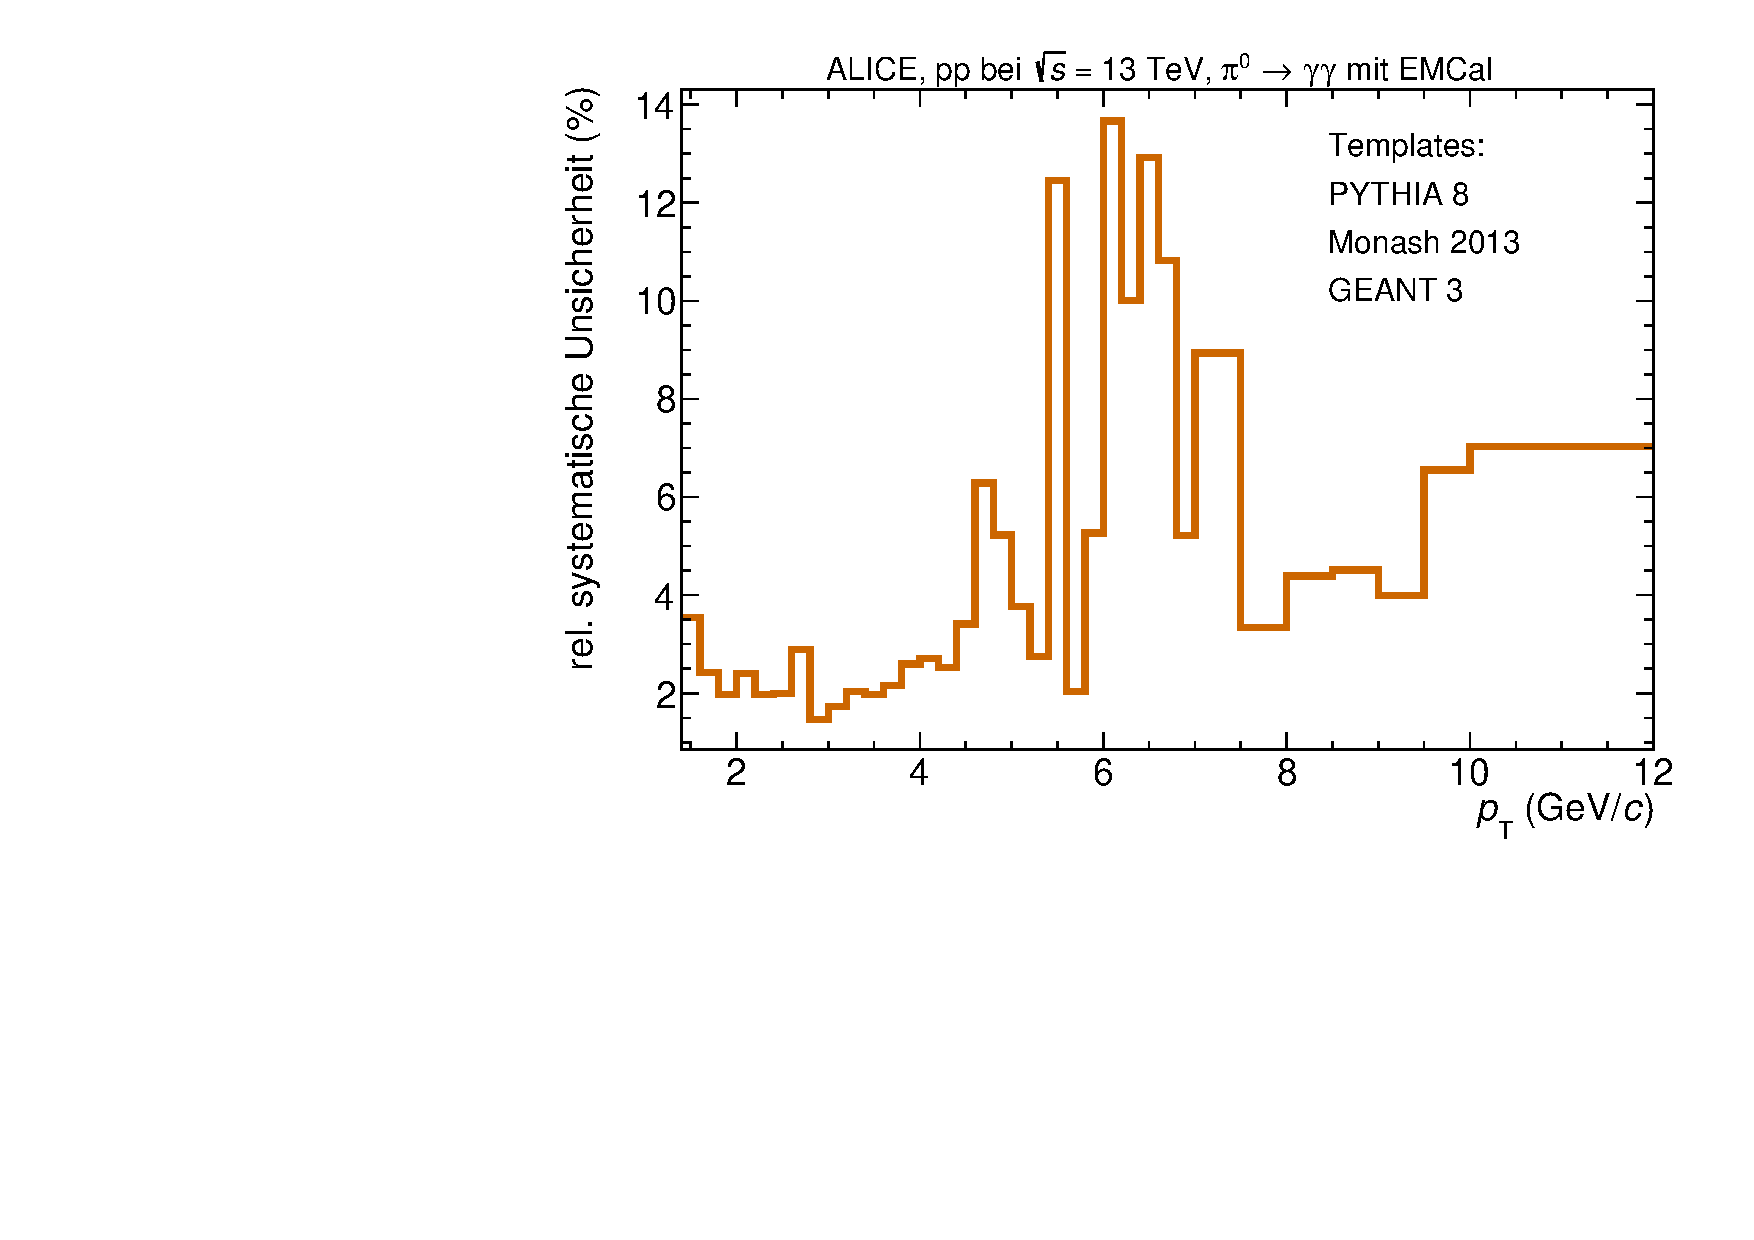
\includegraphics[width=.65\linewidth]{SystematischeUnsicherheit_Data_2016.pdf}
\caption{Gesamte relative systematische Unsicherheit des korrigierten $\pi^ {0}$-Spektrums.}
\label{fig:SysUncer}
\end{figure}
\newline
Zur Bestimmung der systematischen Unsicherheit $\sigma_{i,j}$ einer Variationsart $j$ in einem $p_\text{T}$-Intervall $i$ wird das quadratische Mittel der relativen Abweichungen der $n$ unterschiedlichen Variationen $k$ verwendet.
Es gilt:
\begin{align}
\sigma_{i,j} = \sqrt{\frac{1}{n}\sum_{k=1}^{n}\left(\Delta y_{i,j,k}\right)^{2}}
\end{align}
Die gesamte Systematische Unsicherheit $\sigma_{i}$ in einem $p_\text{T}$-Intervall $i$ ergibt sich aus dem quadratischen Mittelwert der systematischen Unsicherheiten der vier Variationsarten $\sigma_{i,j}$.
\begin{align}
\sigma_{i} = \sqrt{\frac{1}{n}\sum_{j=1}^{n}\left(\sigma_{i,j}\right)^{2}}
\end{align}
\begin{figure}[t!]
\centering
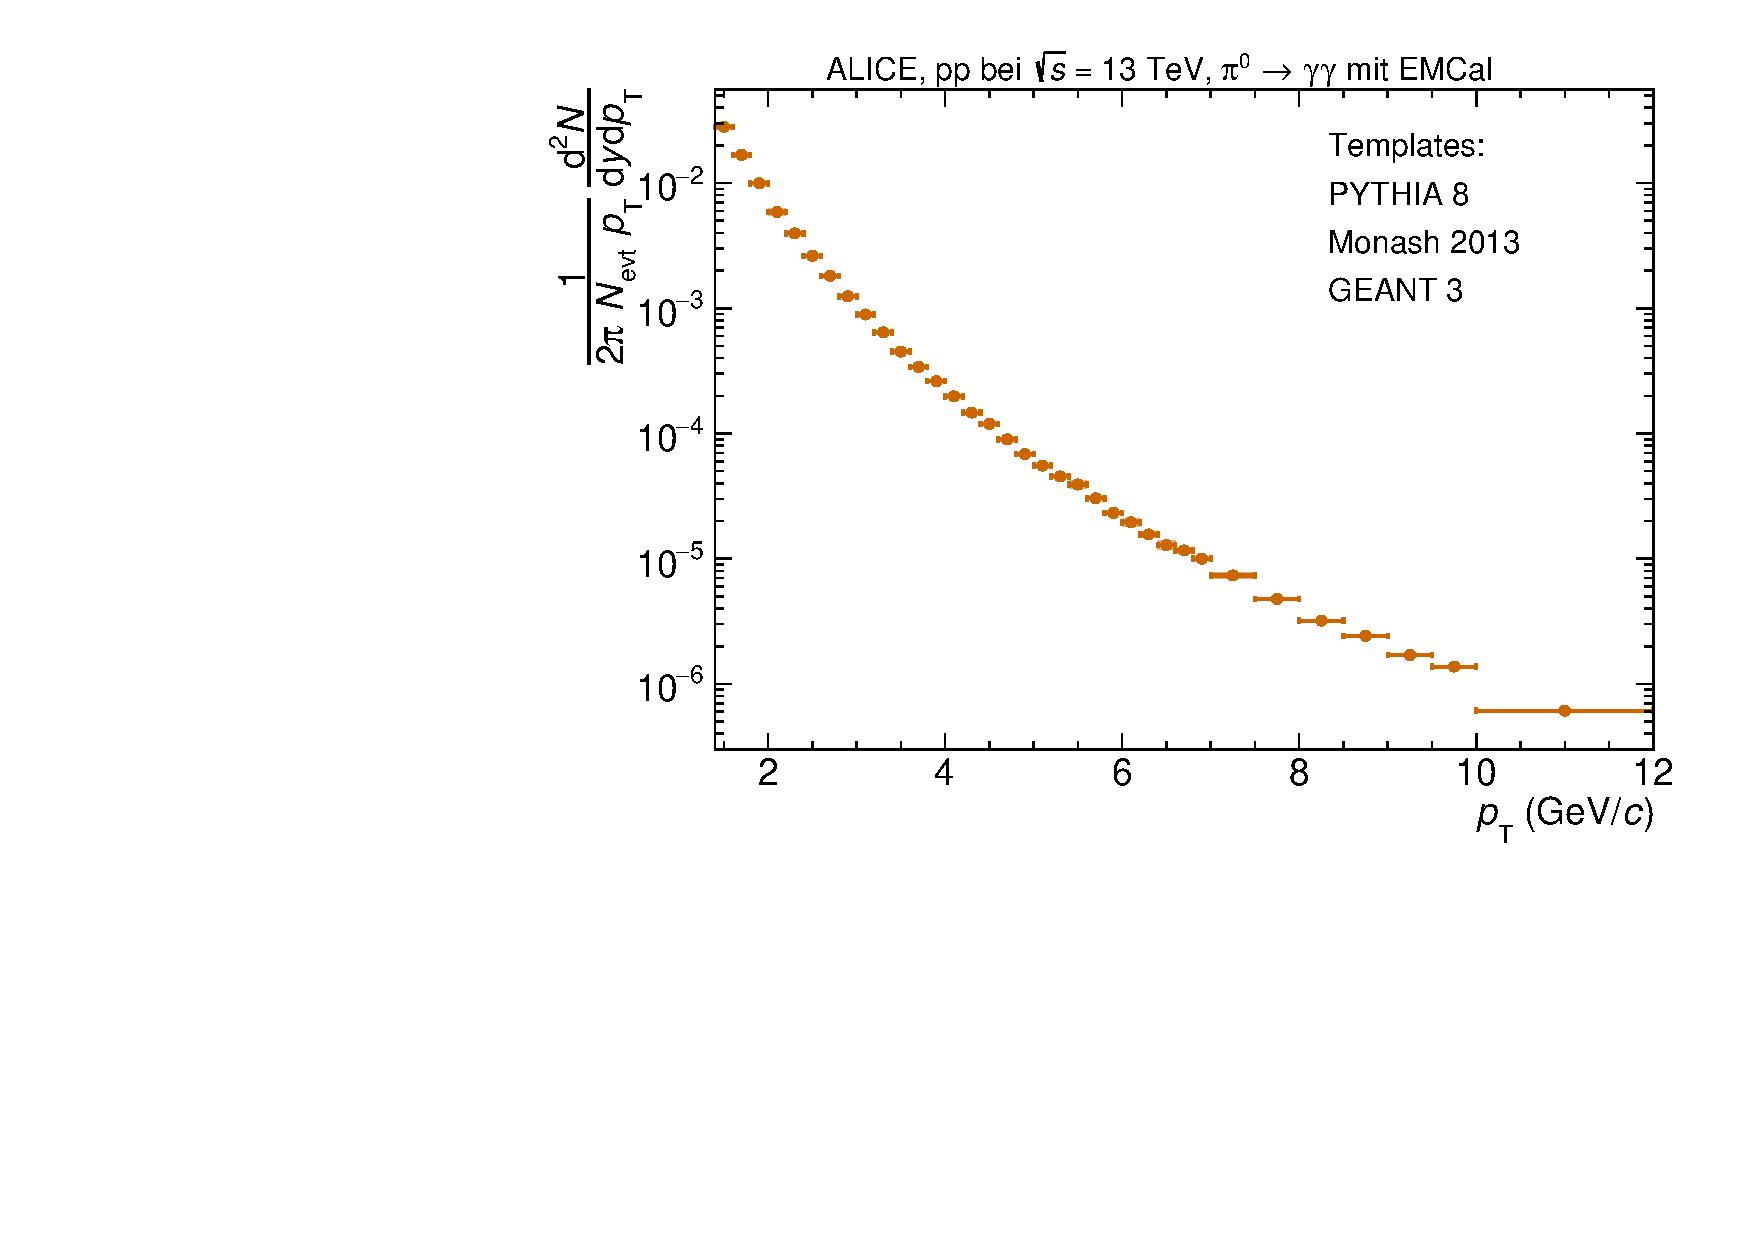
\includegraphics[width=.65\linewidth]{KorrigierterYield_Data_2016.pdf}
\caption{Korrigierter $\pi^{0}$-\textit{Yield} mit systematischen und statistischen Unsicherheiten.}
\label{fig:KorrYield}
\end{figure}
\newline
